\chapter{Risultati}
\bigskip

\section{Risultati del modello lineare}
\bigskip

Per valutare le performance del modello lineare, oltre ai sistemi classici come l'\textit{errore quadratico medio}, abbiamo 
cercato di misurare con che precisione il modello tende a predire il picco influenzale, cioè la settimana con la massima 
incidenza della patologia nella popolazione italiana. Come si può notare dalla Tabella \ref{tab:models_results}, nella metà 
delle stagioni influenzali il modello lineare predice il picco entro una settimana indicata dai dati InfluNet; inoltre, nelle 
stagioni 2008-2009, 2011-2012 e 2014-2015 il picco è previsto correttamente. Negli altri quattro casi il modello lineare 
tende ad anticipare la settimana del picco (stagioni 2007-2008, 2010-2011 e 2013-2014).
\bigskip

Il modello lineare possiede una buona capacità predittiva anche nel caso della stagione influenzale 2009-2010, che fu 
particolarmente grave poiché ci fu una vera e propria epidemia causata dalla varietà H1N1 del virus influenzale. Il picco in 
questo caso è spostato verso le ultime settimane del 2009 (dalla numero 42 alla 52) e non corrisponde all'andamento 
classico della patologia (si nota molto bene dalla Figura \ref{fig:ch_2_ILI_levels}). Inoltre, quell'anno c'era stata una 
grande copertura mediatica riguardo all'epidemia, cosa che avrebbe potuto in qualche modo aggiungere rumore ai dati del 
dataset. Nonostante ciò, il modello riesce a prevedere il picco della stagione correttamente (con uno scarto di una 
settimana).
\bigskip

Abbiamo anche cercato di individuare quali feature siano più importanti per la previsione dei valori di incidenza. Ci siamo 
soffermati su quelle voci di Wikipedia che sono presenti più volte in tutti i modelli e quali di esse avessero il più grande 
peso $\beta_i$ associato. Attraverso l'utilizzo di LASSO abbiamo potuto ridurre considerevolmente il numero di feature che 
effettivamente giocano un ruolo nella previsione dell'incidenza, infatti, da 470 feature, i modelli ne andavano 
ad utilizzare in media 111 (con utilizzare si intende che veniva assegnato loro un peso $\beta_i \neq 0$). 
\bigskip

La Tabella \ref{tab:models_features} mostra le prime 5 feature con peso medio maggiore e in quanti modelli 
esse siano presenti. Come si può notare, sono voci di Wikipedia legate ai sintomi influenzali (la voce con più alto 
peso medio riguarda la patologia \textit{Febbre}). Poiché quasi nel 100\% dei modelli abbiamo le stesse feature, e poiché 
esse danno il contributo più grande nel determinare il livello di incidenza influenzale, possiamo supporre che anche 
l'andamento delle pageview di queste voci rispecchi l'andamento dei dati InfluNet e che quindi pageview ed InfluNet siano in 
qualche modo correlati.
\bigskip

Questa relazione è facilmente visibile ad esempio nella stagione influenzale 2012-2013, come ci mostra la Figura 
\ref{fig:ch_3_correlation_linear}. Se osserviamo l'andamento delle pageview di alcune delle voci della Tabella 
\ref{tab:models_features} rispetto all'incidenza ILI, si può notare come il loro valore inizi ad aumentare esattamente 
nello stesso periodo in cui anche l'incidenza della patologia aumenta. Questa relazione si può osservare anche nelle stagioni 
influenzali 2009-2010 e 2011-2012.
\bigskip

Per verificare che questa relazione tra le pageview e l'incidenza ILI in Italia si presenti solo con pagine legate all'ambito 
medico, in particolare con pagine legate alla patologia influenzale, abbiamo provato ad 
utilizzare il dataset formato da voci estratte casualmente da Wikipedia per allenare il modello lineare, con le stesse 
modalità con cui abbiamo usato quello reale. Come ci aspettavamo, utilizzando le pagine casuali, il modello non riesce ad 
effettuare previsioni coerenti con InfluNet. In certe stagioni influenzali, il modello non riesce neppure a convergere ad una 
soluzione e molto spesso alla quasi totalità delle 470 feature non viene assegnato nessun peso $\beta_i$ diverso da zero. Ciò 
significa che probabilmente non esiste una relazione lineare tra le pageview del dataset casuale e l'incidenza InfluNet, a 
differenza di ciò che accade con il dataset formato da pagine di categoria medica.
\bigskip

\begin{table}[p]
\centering
\begin{adjustbox}{max width=\textwidth}
\begin{tabular}{|c|c|c|c|c|c|}
\hline
\rowcolor[HTML]{EFEFEF} 
\textbf{Stagione Influenzale} & \textbf{Picco IN (Settimana)} & \textbf{Picco M (Settimana)} & \textbf{Picco IN} & \textbf{Picco M} & \textbf{MSE}   \\ \hline
\multicolumn{6}{|c|}{\cellcolor[HTML]{EFEFEF}Modello Lineare} \\ \hline
\textit{2007-2008}            & \textit{5}                          & \textit{1}                    & \textit{7.21}           & \textit{1.64}     & \textit{11.00} \\ \hline
\rowcolor[HTML]{FFFFFF} 
\textit{2008-2009}            & \textit{4}                          & \textit{4}                    & \textit{8.23}           & \textit{6.64}     & \textit{4.43}  \\ \hline
\rowcolor[HTML]{FFFFFF} 
\textit{2009-2010}            & \textit{46}                         & \textit{45}                   & \textit{12.92}          & \textit{10.89}    & \textit{5.02}  \\ \hline
\rowcolor[HTML]{FFFFFF} 
\textit{2010-2011}            & \textit{5}                          & \textit{4}                    & \textit{11.04}          & \textit{14.80}    & \textit{7.35}  \\ \hline
\rowcolor[HTML]{FFFFFF} 
\textit{2011-2012}            & \textit{5}                          & \textit{5}                    & \textit{9.64}           & \textit{7.99}     & \textit{1.29}  \\ \hline
\rowcolor[HTML]{FFFFFF} 
\textit{2012-2013}            & \textit{6}                          & \textit{5}                    & \textit{9.99}           & \textit{11.95}    & \textit{2.67}  \\ \hline
\rowcolor[HTML]{FFFFFF} 
\textit{2013-2014}            & \textit{6}                          & \textit{3}                    & \textit{6.67}           & \textit{13.80}    & \textit{7.38}  \\ \hline
\rowcolor[HTML]{FFFFFF} 
\textit{2014-2015}            & \textit{4}                          & \textit{4}                    & \textit{10.87}          & \textit{5.11}     & \textit{7.18}  \\ \hline
\rowcolor[HTML]{FFFFFF} 
\textit{2015-2016}            & \textit{8}                          & \textit{5}                    & \textit{6.14}           & \textit{5.59}     & \textit{2.55}  \\ \hline
\rowcolor[HTML]{EFEFEF} 
\multicolumn{6}{|c|}{\cellcolor[HTML]{EFEFEF}Modello di Poisson} \\ \hline
\textit{2007-2008}            & \textit{5}                          & \textit{1}                    & \textit{7.21}           & \textit{1.01}     & \textit{13.02}    \\ \hline
\rowcolor[HTML]{FFFFFF} 
\textit{2008-2009}            & \textit{4}                          & \textit{4}                    & \textit{8.23}           & \textit{5.78}     & \textit{3.31}     \\ \hline
\rowcolor[HTML]{FFFFFF} 
\textit{2009-2010}            & \textit{46}                         & \textit{45}                   & \textit{12.92}          & \textit{1090.86}  & \textit{44764.56} \\ \hline
\rowcolor[HTML]{FFFFFF} 
\textit{2010-2011}            & \textit{5}                          & \textit{6}                    & \textit{11.04}          & \textit{59.16}    & \textit{147.97}   \\ \hline
\rowcolor[HTML]{FFFFFF} 
\textit{2011-2012}            & \textit{5}                          & \textit{5}                    & \textit{9.64}           & \textit{8.57}     & \textit{1.27}     \\ \hline
\rowcolor[HTML]{FFFFFF} 
\textit{2012-2013}            & \textit{6}                          & \textit{8}                    & \textit{9.99}           & \textit{8.45}     & \textit{6.25}     \\ \hline
\rowcolor[HTML]{FFFFFF} 
\textit{2013-2014}            & \textit{6}                          & \textit{3}                    & \textit{6.67}           & \textit{16.48}    & \textit{6.15}     \\ \hline
\rowcolor[HTML]{FFFFFF} 
\textit{2014-2015}            & \textit{4}                          & \textit{5}                    & \textit{10.87}          & \textit{4.95}     & \textit{9.73}     \\ \hline
\rowcolor[HTML]{FFFFFF} 
\textit{2015-2016}            & \textit{8}                          & \textit{7}                    & \textit{6.14}           & \textit{5.23}     & \textit{2.64}     \\ \hline
\end{tabular}
\end{adjustbox}
\caption{\textit{Per ogni stagione influenzale e per ogni modello sono stati registrati: la settimana in cui è presente il 
picco massimo di incidenza ILI indicato dai dati InfluNet, la settimana con il picco massimo di incidenza predetto dai 
modelli, il valore dell'incidenza del picco massimo di InfluNet, il valore dell'incidenza del picco massimo predetto dai modelli e l'MSE (Mean Squared Error), per misurare le prestazioni dei modelli nelle varie stagioni influenzali. Con la sigla IN si intende il valore indicato dai dati InfluNet, mentre con M si indica il valore predetto dai modelli.}}
\label{tab:models_results}
\end{table}

\begin{table}[p]
\centering
\begin{adjustbox}{max width=\textwidth}
\begin{tabular}{|l|l|l|}
\hline
\rowcolor[HTML]{EFEFEF} 
\textbf{Feature}                            & \textbf{Peso Medio} & \textbf{Modelli in cui è presente} \\ \hline
\rowcolor[HTML]{EFEFEF} 
\multicolumn{3}{|c|}{\cellcolor[HTML]{EFEFEF}Modello Lineare} \\ \hline
\textit{Febbre}                             & \textit{13.11}      & \textit{9/9}                                            \\ \hline
\textit{Influenza}                          & \textit{4.71}       & \textit{9/9}                                            \\ \hline
\textit{Bronchite}                          & \textit{4.64}       & \textit{9/9}                                            \\ \hline
\textit{Influenzavirus\_A\_sottotipo\_H1N1} & \textit{3.98}       & \textit{8/9}                                            \\ \hline
\textit{Polipnea}                           & \textit{3.01}       & \textit{9/9}                                            \\ \hline
\rowcolor[HTML]{EFEFEF} 
\multicolumn{3}{|c|}{\cellcolor[HTML]{EFEFEF}Modello di Poisson} \\ \hline
\textit{Pagina principale}                      & \textit{0.52}                              & \textit{9/9}                                              \\ \hline
\textit{Febbre ricorrente}                      & \textit{0.07}                              & \textit{9/9}                                              \\ \hline
\textit{Vaccino per la febbre tifoide}          & \textit{0.06}                              & \textit{2/9}                                              \\ \hline
\textit{Stimmate\_(medicina)}                   & \textit{0.05}                              & \textit{8/9}                                              \\ \hline
\textit{Virus dell'encefalite di Murray Valley} & \textit{0.05}                              & \textit{2/9}                                              \\ \hline
\end{tabular}
\end{adjustbox}
\caption{\textit{Tabella indicante le feature utilizzate dai modelli ordinate per il loro peso medio.}}
\label{tab:models_features}
\end{table}

Osservando i grafici successivi (Figura \ref{fig:appendix_linear}), si osserva come il modello lineare sia più efficace 
nelle stagioni influenzali che vanno dalla 2008-2009 fino alla 2012-2014, mentre si comporta relativamente peggio nelle 
stagioni 2007-2008, 2014-2015 e 2015-2016. Le basse prestazioni possono essere spiegati nel seguente modo: 
\begin{itemize}
\item Nel caso della stagione 2007-2008 alcune delle voci utilizzate dal modello non erano ancora ancora presenti come 
pagine di Wikipedia, quindi il valore delle pageview settimanali per la stagione 2007-2008 per queste feature non è 
disponibile. Infatti, su 470 feature, 184 sono "nulle", mentre delle 51 feature utilizzate dal modello 18 di queste hanno 
valori sempre uguali a zero nel dataset che copre l'arco di tempo 2007-2008. Probabilmente, a causa di ciò il modello ha 
stimato valori di incidenza ILI più bassi del normale, poiché non aveva sufficienti informazioni per dare una previsione 
corretta;
\item Nel caso delle stagioni 2014-2015 e 2015-2016, la causa può essere imputata principalmente alla mancanza di una 
variazione significativa dei valori delle pageview per le voci selezionate dal modello. In sostanza, a differenza del 
2012-2013, in cui l'andamento delle voci seguiva quello dell'incidenza ILI, nel 2014-2015 e 2015-2016 ciò non succede. 
Questo potrebbe essere causato dalla mancanza nel dataset di informazioni riguardanti gli accessi tramite dispositivi mobile 
che, se aggiunte, potrebbero migliorare le prestazioni (che come si è detto nel capitolo precedente, ora sono maggioritarie 
rispetto ai semplici accessi via desktop).
\end{itemize}

\begin{figure}[ht]
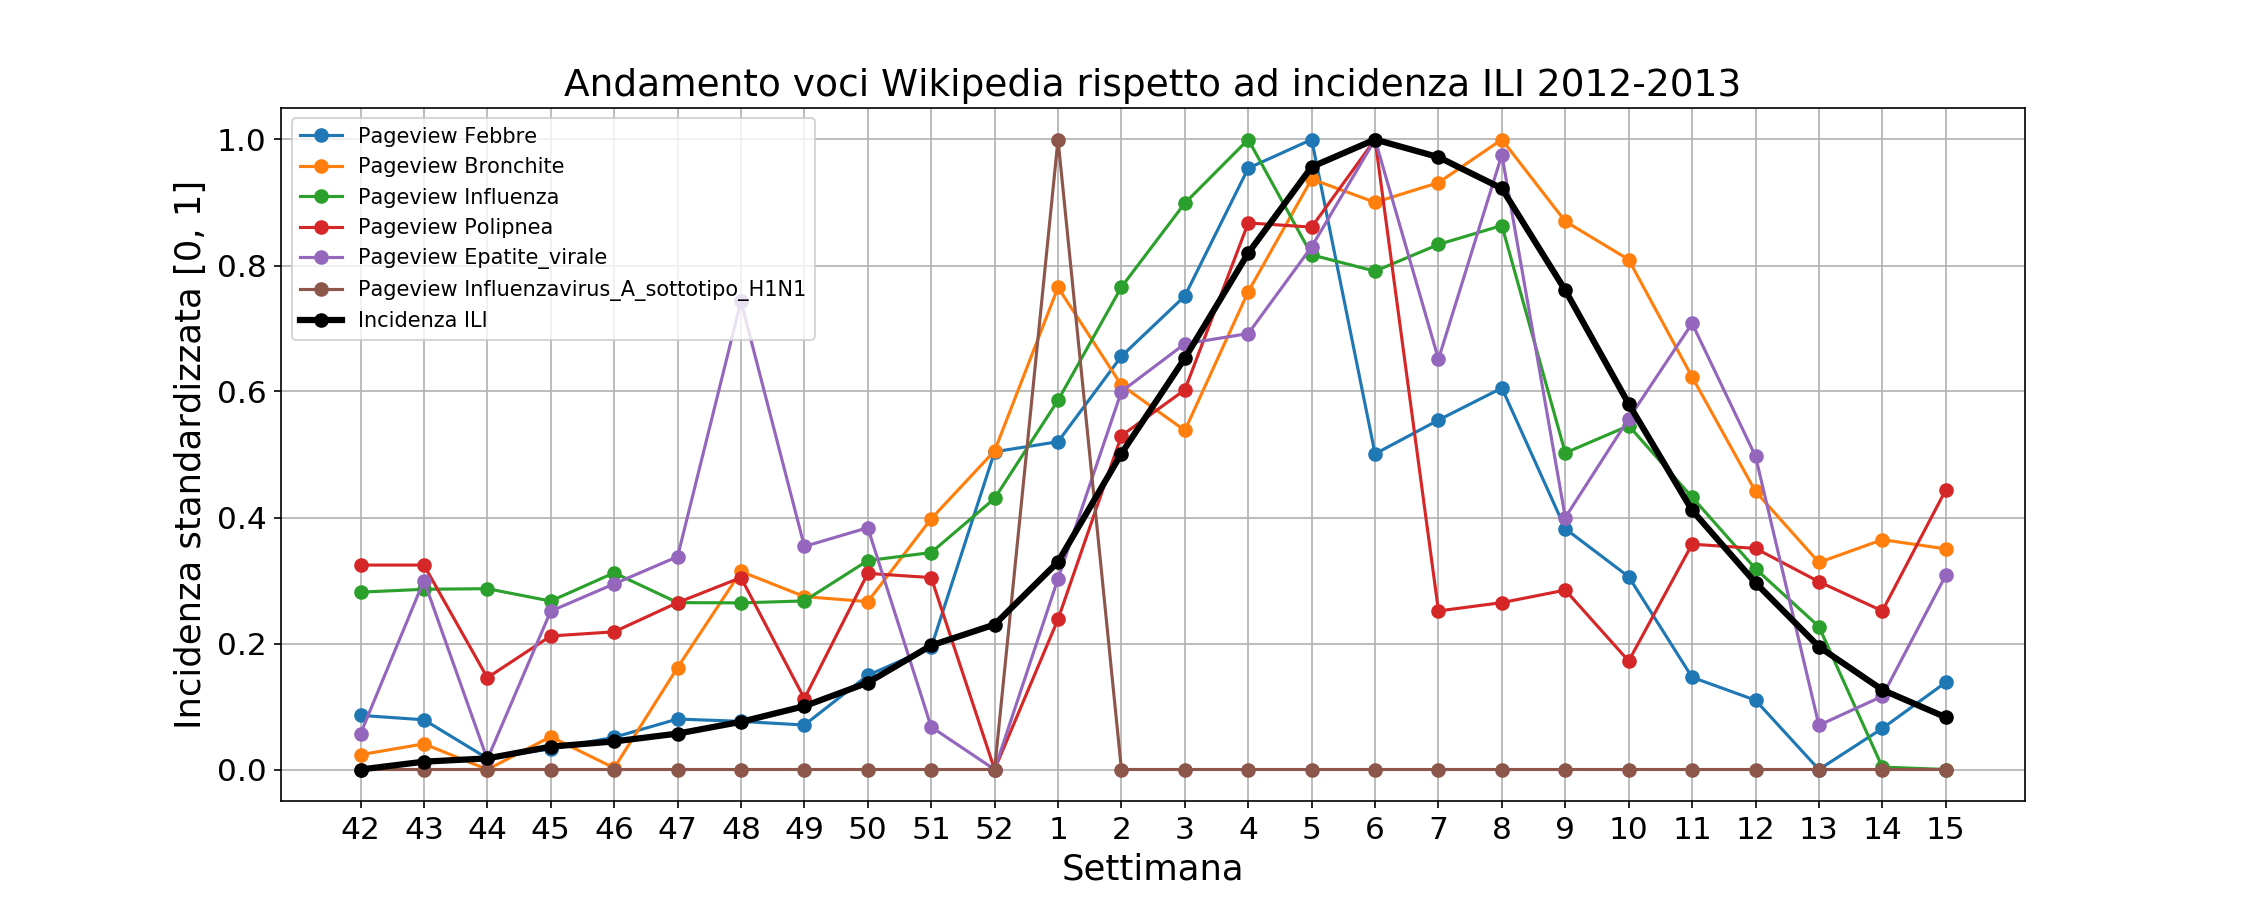
\includegraphics[width=\textwidth]{chapter_3_correlation_linear}
\caption{\textit{Variazione del valore di alcune feature rispetto all'incidenza ILI (i valori per essere comparati sono stati normalizzati nell'intervallo [0,1]).}}
\label{fig:ch_3_correlation_linear}
\centering
\end{figure}

\section{Risultati del modello di Poisson}
\bigskip

Per valutare le prestazioni del modello di Poisson abbiamo proceduto come abbiamo fatto per il modello lineare, osservando 
con quanta efficacia vengono previsti i picchi influenzali, il loro valore e l'andamento generale dell'incidenza ILI. 
Nonostante nel paper di riferimento \cite{McIver2014} l'utilizzo di un modello generalizzato si sia rivelato efficace e 
adatto a stimare i livelli di ILI, per l'Italia il modello di Poisson non ha mostrato significativi miglioramenti rispetto al 
modello lineare, anzi in certi casi ha mostrato un calo di prestazioni. Come mostra la Tabella 
\ref{tab:models_results}, pur riuscendo a stimare il picco influenzale (con uno scarto di una settimana) in cinque 
stagioni su nove, il modello tende in alcuni casi a sovrastimare in maniera abbondante l'incidenza del picco.
\bigskip

Riguardo invece alle feature utilizzate, osservando la Tabella \ref{tab:models_features}, si nota come il modello di 
Poisson tenda a dare maggior peso a voci di Wikipedia che poco hanno a che fare con i sintomi della patologia influenzale. 
Inoltre, i pesi assegnati hanno un entità molto minore rispetto a quelli del modello lineare e  
l'andamento delle feature rispetto al valore dell'incidenza ILI non ha una corrispondenza così netta (Figura 
\ref{fig:ch_3_correlation_poisson}).
\bigskip

Il modello è anche poco resistente agli \textit{outliers} presenti nel dataset di Wikipedia. Infatti, come si nota dai 
grafici in Figura \ref{fig:appendix_poisson}, nella sesta settimana del 2011 e
nella terza e nona settimana del 2014, il modello stima dei valori di incidenza ILI molto elevati, rispetto a quanto indicato 
dai dati Influnet. Questi sono per lo più causati da voci di Wikipedia che in quelle specifiche settimane hanno ricevuto un 
totale di visite che si discosta in maniera evidente dalla loro media settimanale (probabilmente a causa di alcuni bot).
\bigskip 

Per confermare comunque che questi risultati si ottengono soltanto quando si analizzano le voci di categoria medica di 
Wikipedia, abbiamo provato ad utilizzare il dataset composto da voci casuali e l'esito è stato lo stesso di quello ottenuto 
con il modello lineare. Il modello generalizzato non riesce a prevedere con sufficiente accuratezza ne i picchi influenzali, 
ne il normale andamento dell'incidenza ILI. 
\bigskip

Il modello di Poisson ha lo stesso comportamento del modello lineare per quanto riguarda le stagioni influenzali 2007-2008, 
2014-2015 e 2015-2016. Le basse prestazioni in quei casi possono essere addotte alle stesse motivazioni presentate per il 
modello lineare, cioè la mancanza di una parte significativa delle \textit{page view} dal dataset e con un numero troppo 
elevato di predittori nulli.
\bigskip

Un altra motivo per cui le prestazioni non sono ottimali potrebbero essere il fatto che la regressione di Poisson assume 
che la variabile aleatoria dipendente (cioè in questo caso il valore di incidenza ILI) segua la distribuzione di Poisson. 
Questo porta con se una condizione abbastanza restrittiva che implica che la sua media e la sua varianza devono essere 
uguali, cosa che non è sempre vera nei dataset reali. Infatti, si può notare come in tutte le stagioni influenzali 
l'incidenza ILI tenda a seguire una distribuzione normale (che quindi è più adatta ad essere prevista con un semplice modello 
lineare) rendendo quindi difficile l'utilizzo di questo metodo per costruire un modello predittivo.
\bigskip

\begin{figure}[h]
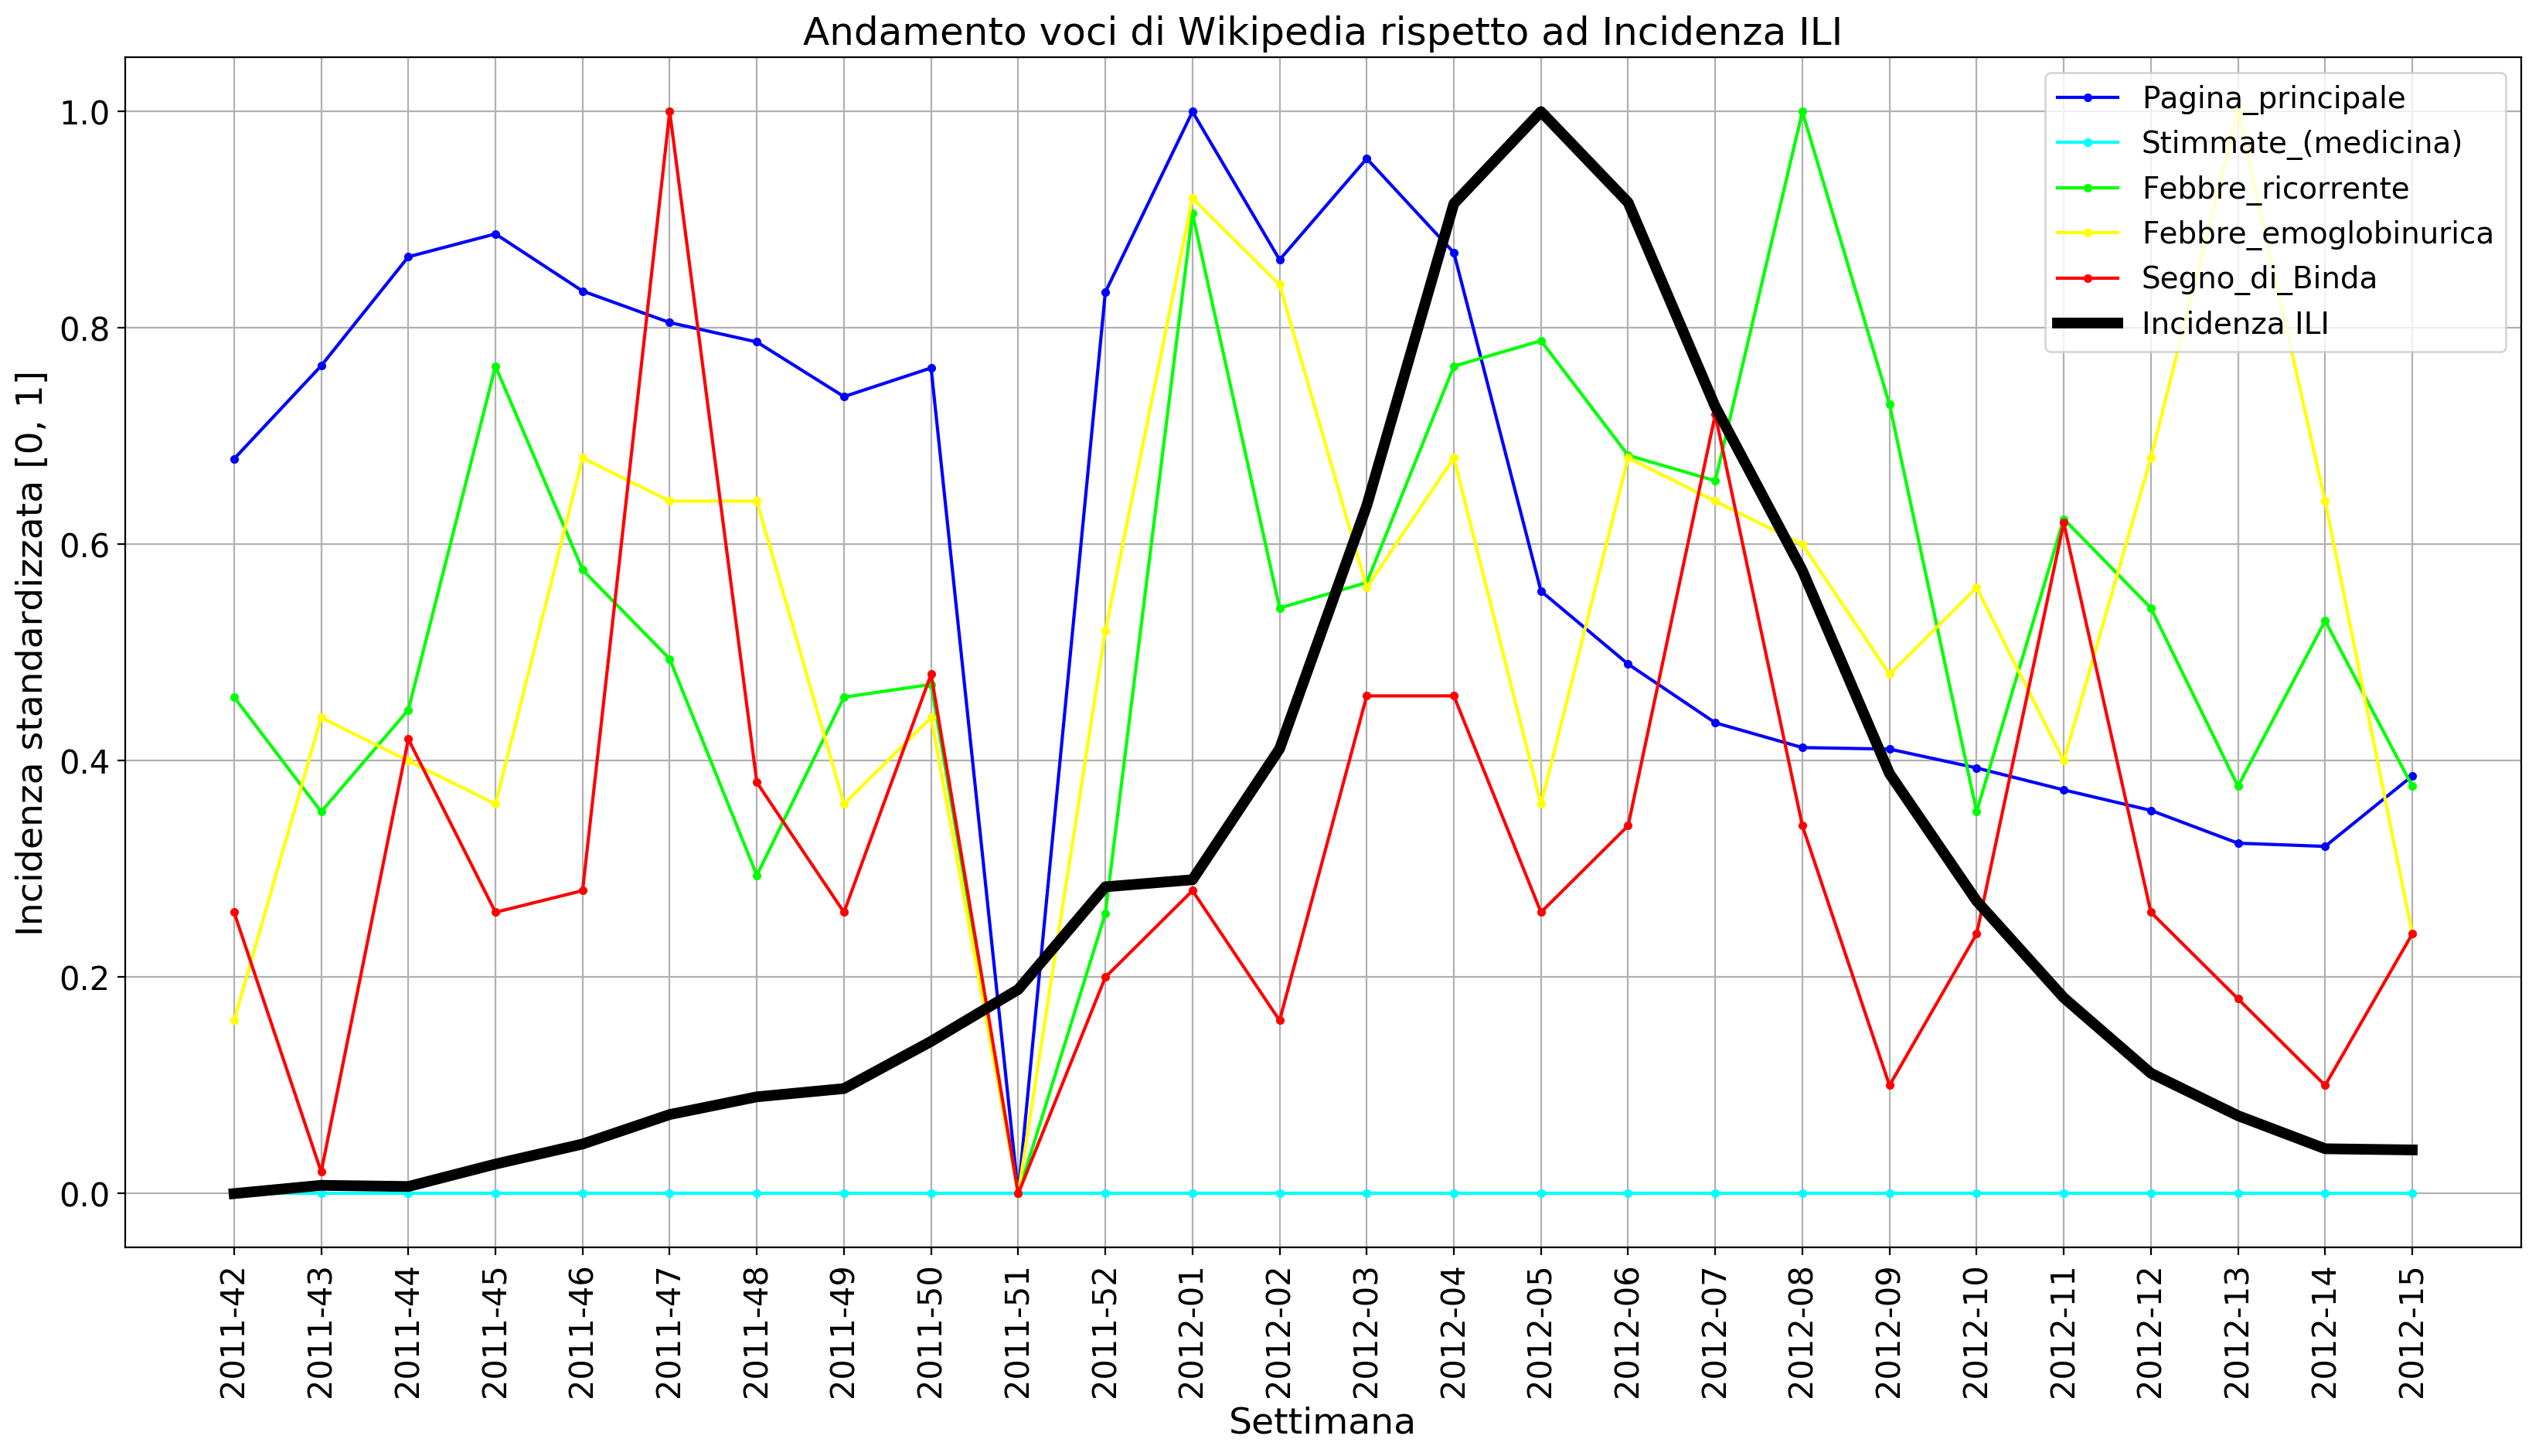
\includegraphics[width=\textwidth]{chapter_3_correlation_poisson}
\caption{\textit{Variazione del valore delle prime 5 feature rispetto all'incidenza ILI (i valori per essere comparati sono stati normalizzati nell'intervallo [0,1]).}}
\label{fig:ch_3_correlation_poisson}
\centering
\end{figure}

\clearpage